An important correctness issue of TLB shootdown seems promising to be studied. The GPU MMU design handles TLB flushes similarly to the CPU MMU. Particularly when the register which stored the pointer to the page table is written, the GPU MMU is notified via inter-processor communication and all of the GPU TLBs are flushed. This is a rare event, usually happens between two different kernels. A more common case is when a page-fault occurs and a new page is brought to GPU memory, all TLBs need to be flushed because the MMU does not know which TLB has stale translation infomation.

Mechanisms to reduce the cost of TLB shootdowns on CPUs, and emerging heterogeneous memory systems, have attracted significant attention over the last decade. This is due to the rising cost of TLB shootdowns, especially as core counts continue to scale and heterogeneous memory makes its way into mainstream systems. Previous work by Agarwal et al. have studied on mechanisms to reduce the occurrence of TLB shootdowns on a CPU-GPU system. Reducing the cost for translation coherence on virtualized systems has also been studied.

With UVM Smart simulation framework, it would not be hard to gain the insight of TLB performance. Therefore, we run an experiment in terms of GPU TLB shootdown granularity. We want to justify the positive impact of advanced TLBs. The result shows that the TLB shootdown penalty is not significantly varied among different shootdown granularity.


   \begin{figure}[!htb]
      \centering
      \setlength{\abovecaptionskip}{6pt plus 1pt minus 1pt}
      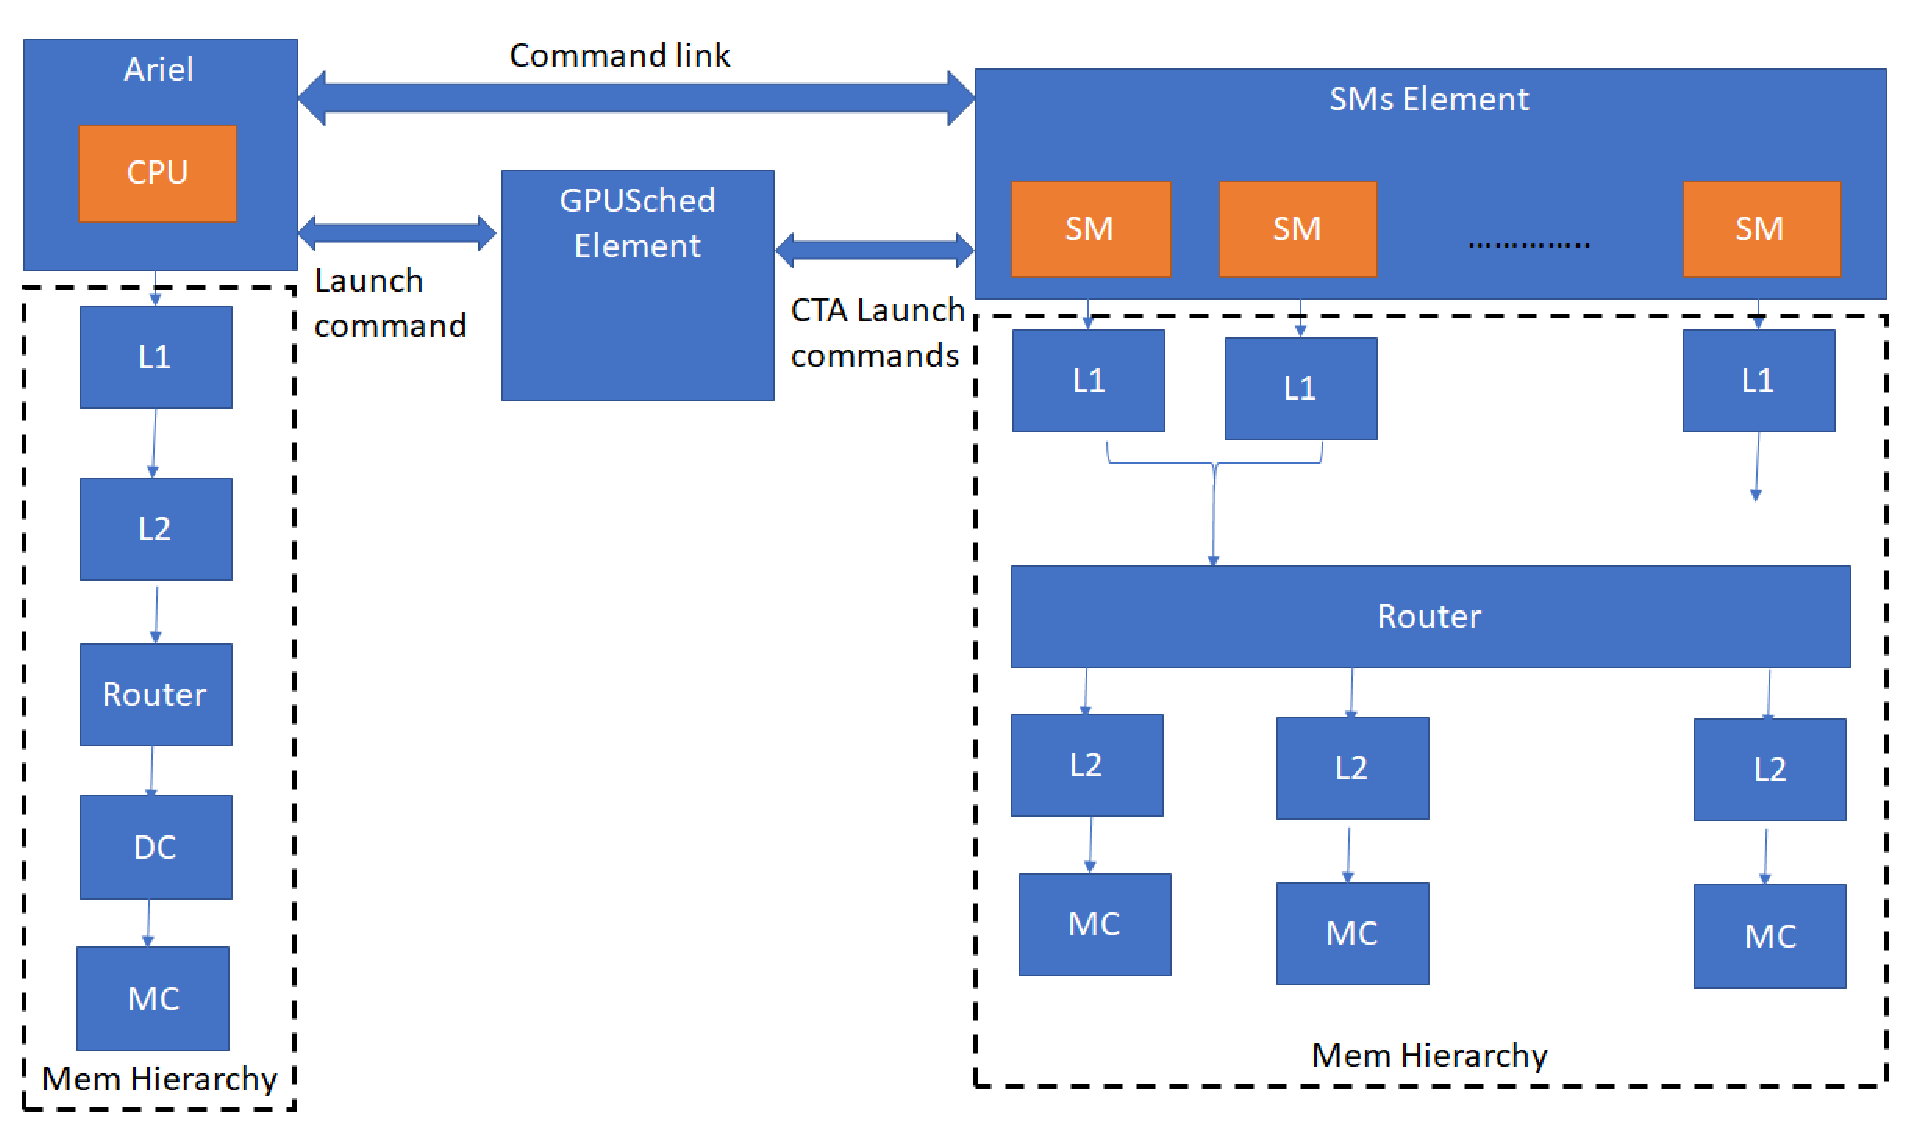
\includegraphics[width=.90\textwidth,keepaspectratio]{figures/3_1.eps}
      \captionsetup{width=.75\textwidth}
      \caption{Timing and memory model for SMs component}
      \label{fig:gpu_mem_model}
   \end{figure}
